\section*{马尔科夫场}

\begin{frame}
	\centerline{\textbf{\Large{马尔科夫场}}} 
	~\\
	\centerline{\large{王方正}}
\end{frame}

\subsection*{模型定义}
\begin{frame}
	马尔科夫随机场,又称为概率无向图模型,是一个可以由无向图表示的联合概率分布。
\end{frame}

\begin{frame}

	\begin{block}{图}
		图是由结点及连接结点的边组成的集合。结点和边分别记作$v$和$e$,结点和边的集合分别记作$V$和$E$,图记作$G=(V,E)$。\\
		无向图是指边没有方向的图。
	\end{block}

	\begin{block}{概率图模型}
		概率图模型(PGM)是由图表示的概率分布。设有联合概率分布$P(Y)$,$Y\in\mathcal{Y}$是一组随机变量。由无向图$G=(V,E)$表示概率分布,即在图$G$中,结点$v\in V$表示一个随机变量$Y_v$,$Y=(Y_v)_{v\in V}$;边$e\in E$表示随机变量之间的概率依赖关系。
	\end{block}

\end{frame}

\begin{frame}
	马尔可夫性:三者等价
	
	\begin{itemize}
		\item 成对马尔可夫性:$P(Y_u,Y_v|Y_O)=P(Y_u|Y_O)P(Y_v|Y_O)$
		\item 局部马尔可夫性:$P(Y_v,Y_O|Y_W)=P(Y_v|Y_W)P(Y_O|Y_W)$
		\item 全局马尔可夫性:$P(Y_A,Y_B|Y_C)=P(Y_A|Y_C)P(Y_B|Y_C)$
	\end{itemize}

\end{frame}

\begin{frame}

	\begin{figure}[htbp]
		\centering
		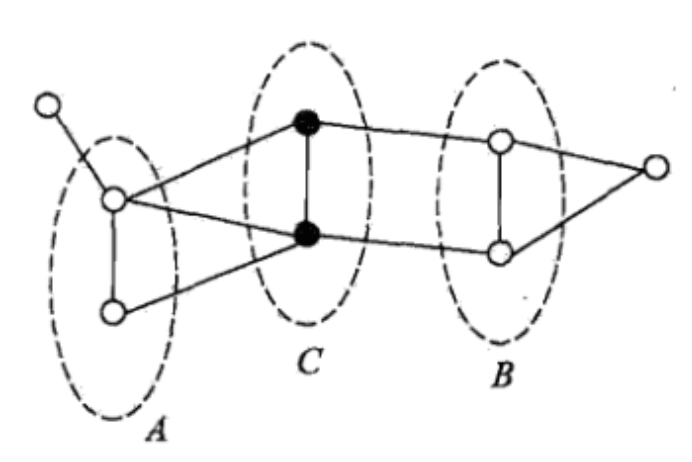
\includegraphics[scale=0.6]{pic/1-1.png}
		\caption{局部马尔可夫性}
		\label{1-001}
	\end{figure}

\end{frame}

\begin{frame}

	\begin{figure}[htbp]
		\centering
		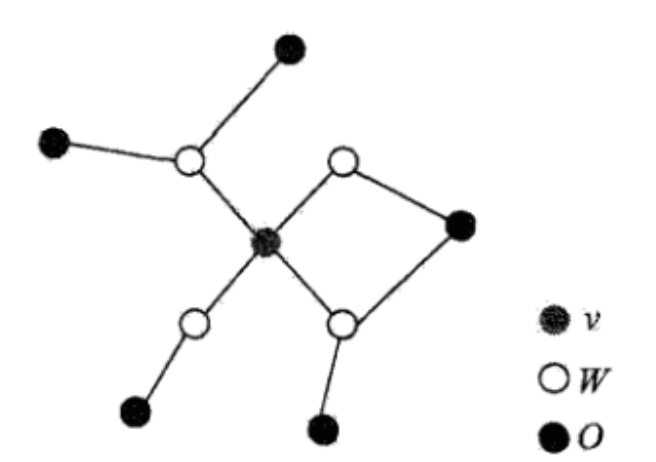
\includegraphics[scale=0.6]{pic/1-2.png}
		\caption{全局马尔可夫性}
		\label{1-002}
	\end{figure}

\end{frame}

\begin{frame}

	\begin{block}{概率无向图模型}
		设有联合概率分布$P(Y)$ ,由无向图$G=(V,E)$表示,在图$G$中,结点表示随机变量,边表示随机变量之间的依赖关系。如果联合概率分布$P(Y)$满足成对、局部或全局马尔可夫性,就称此联合概率分布为概率无向图模型或马尔可夫随机场。
	\end{block}

\end{frame}

\subsection*{因子分解}

\begin{frame}

	\begin{block}{团}
		无向图$G$中任何两个结点均有边连接的结点子集称为团。
	\end{block}
	
	\begin{block}{最大团}
		若$C$是无向图$G$的一个团,并且不能再加进任何一个$G$的结点使其成为一个更大的团,则称此$C$为最大团。
	\end{block}

\end{frame}

\begin{frame}

	\begin{figure}[htbp]
		\centering
		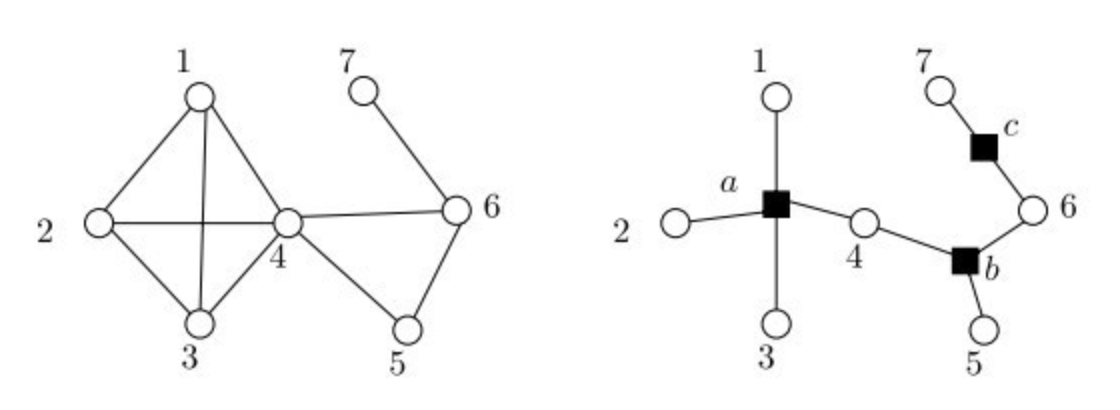
\includegraphics[scale=0.6]{pic/1-3.png}
		\caption{无向图与因子图}
		\label{1-003}
	\end{figure}

\end{frame}

\begin{frame}

	将概率无向图模型的联合概率分布表示为其最大团上的随机变量的函数的乘积形式的操作,称为概率无向图模型的因子分解。具体公式为:
	$$P(Y)=\frac{1}{Z}\prod_{C}\Psi_{C}(Y_C)$$
	其中,Z是规范化因子,由式
	$$Z=\sum_{Y}\prod_{C}\Psi_{C}(Y_C)$$
	给出。规范化因子保证$P(Y)$构成一个概率分布。\\
	函数$\Psi_{C}(Y_C)$称为势函数,通常定义为指数函数:
	$$\Psi_{C}(Y_C)=exp^{-E(Y_C)}$$
	势函数的作用是刻画变量之间的相关关系,它是非负函数,并且在所偏好的变量取值上有较大函数值。

\end{frame}

\subsection*{应用}

\begin{frame}

	\begin{figure}[htbp]
		\centering
		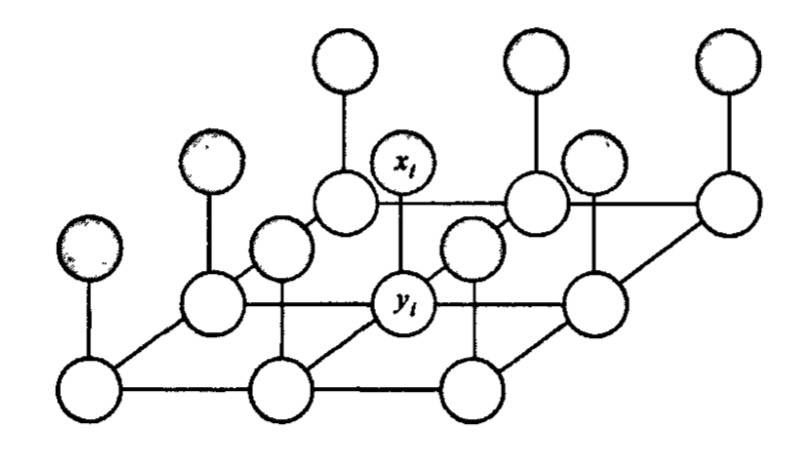
\includegraphics[scale=0.6]{pic/1-4.png}
		\caption{Pairwise MRF 模型}
		\label{1-004}
	\end{figure}

\end{frame}









